\documentclass[10pt,twocolumn]{article}
\usepackage{amsmath}
\usepackage{breqn}
\usepackage[brazil]{babel}
\usepackage[utf8]{inputenc}
\usepackage[T1]{fontenc}
\usepackage{geometry}
\usepackage{gensymb}
\usepackage{graphicx}
\usepackage{listings}
\setlength{\parindent}{0em}
\setlength{\parskip}{0.5em}
\geometry{
a4paper,
total={170mm,257mm},
left=15mm,
right=15mm,
top=15mm,
bottom=15mm,
}

\pagenumbering{gobble}

\begin{document}
\textbf{\large Mini EP 4: Overhead ​e ​Starvation ​em Algoritmos para a Seção Crítica}
\vspace{1em}

O objetivo deste mini EP é comparar os algoritmos de bakery e gate, analisando em quais casos cada um deles apresenta o melhor desempenho de acordo com a quantidade de threads e o tamanho da seção crítica. No pacote de entrega, foram incluídos os arquivos \texttt{main.c} e \texttt{statistics.c} com pequenas adaptações. Além disso, foram incluídos quatro arquivos adicionais: \texttt{script.sh, bakery.csv, gate.csv, stats.py}. Para rodar o script, os outros arquivos de código originais são necessários; já \texttt{stats.py} pode ser rodado de forma independente para visualizar os resultados.

A primeira parte da análise consiste em executar testes com o programa \texttt{teste} e verificar se a exclusão mútua é garantida ao remover a primitiva \texttt{__sync_synchronize()}, que é usada após as atribuições de variáveis para ‘forçá-las’ a serem atômicas. Foram feitas 1000 execuções com 100 threads para cada algoritmo. Observou-se que a exclusão mútua é violada em 7\% das execuções do bakery, e em 100\% das execuções do gate. Dois dos possíveis motivos para o algoritmo gate ser completamente sensível à remoção da primitiva são: (i) o gate faz quatro atribuições, enquanto o bakery faz apenas duas; (ii) três das atribuições do gate estão dentro de ifs (sendo que uma delas passa por dois ifs), o que pode gerar algum conflito com branches. Já o algoritmo bakery é pouco sensível à remoção da primitiva, o que indica que, na maior parte dos casos, a instrução de atribuição já é atômica. Entretanto, é preciso garantir atomicidade para todos os casos; logo, \texttt{__sync_synchronize()} é necessário.

A outra parte da análise consiste em colher dados do programa \texttt{main} variando os parâmetros de entrada (número de threads e quantidade de acessos à seção crítica) para observar como eles afetam o tempo de execução (relacionado a overhead) e a distribuição do número de acessos entre threads (relacionada a starvation). O programa \texttt{main} recebe os parâmetros de entrada, executa cada um dos algoritmos 30 vezes e, para cada vez, imprime o tempo gasto e algumas informações estatísticas. Ele foi modificado para receber o algoritmo a ser rodado como um terceiro parâmetro de entrada (0=bakery; 1=gate) e retornar dados que são salvos em arquivos \texttt{.csv} através de \texttt{script.sh}. Variando número de threads em $[10:10:100]$ e acessos à seção crítica em $[3 \cdot 10^6:10^6:10^7]$, foram coletados conjuntos de pontos com os seguintes atributos: num_threads, total_time, running_time, avg_accesses, stddev_accesses.

A partir desses dados, foram construídas as duas projeções ao lado com \texttt{stats.py}. É possível identificar dois clusters distintos em cada imagem. No gráfico de cima, a altura z é o tempo de execução, em nanosegundos. Nota-se que o algoritmo bakery tem maior tempo de execução, e que esse tempo aumenta com o número de threads. Isso indica overhead, e é esperado, já que o protocolo de entrada do bakery calcula o máximo de um vetor de dimensão igual ao número de threads. No gráfico de baixo, a altura z é o desvio padrão da quantidade de acessos das threads. O desvio padrão quantifica o espalhamento dos pontos em torno da média de acessos e pode ser interpretado como uma medida de justiça do algoritmo: quanto maior for o desvio padrão, menos justo é o algoritmo. Pode se observar que o algoritmo gate apresenta valores bem maiores de desvio padrão. Isso significa que algumas threads estão acessando a seção crítica muitas vezes, e outras poucas vezes. Houve casos em que pelo menos uma thread não conseguiu acessar a seção crítica - ou seja, houve starvation.

Dessas análises, pode se concluir que o gate é significativamente mais rápido, e o bakery significativamente mais justo. Em geral, prioriza-se o custo computacional; logo, o algoritmo gate parece mais vantajoso. A escolha de um ou outro, entretanto, depende das especificações da aplicação.

\begin{figure}
  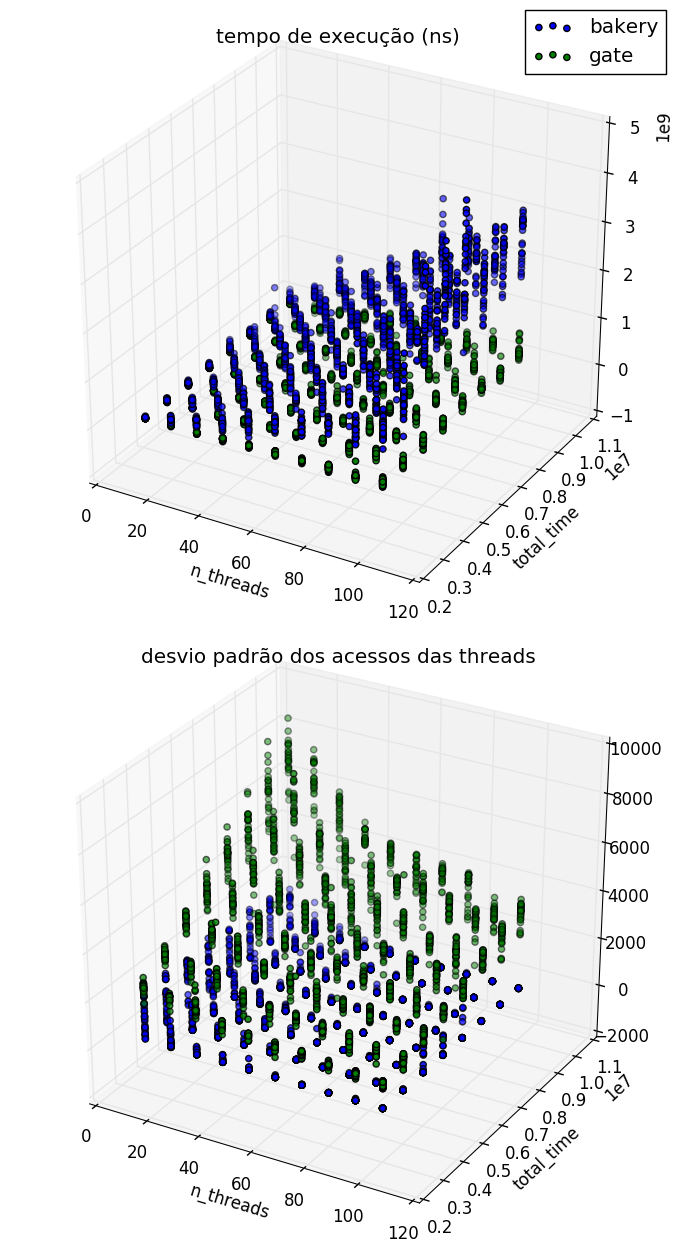
\includegraphics[width=\linewidth]{figure_1.png}
\end{figure}


\end{document}
